\documentclass{article}
\usepackage[utf8]{inputenc}
\usepackage{listings} 
\usepackage{inconsolata} 
\usepackage{blindtext,expdlist} \usepackage{hyperref}

\usepackage{graphicx}
\graphicspath{ {./} }
\usepackage[]{algorithm2e}
\usepackage{amssymb}


% \lstdefinelanguage{CISCO} 
% { 
% sensitive=true, 
% morekeywords=[1]{}, 
% } 


\title{EF513 : Introduction to Music \\Mini Project : Spectrum analysis}
\author{\href{https://gihan.me}{Gihan Jayatilaka}\footnote{\href{mailto:gihanjayatilaka@eng.pdn.ac.lk}{gihanjayatilaka@eng.pdn.ac.lk}} \hspace{1cm} E/14/158}
\date{25/05/2020}
\begin{document}

\maketitle

\section{Implementation :Write a computer program (in Matlab or any other language) to extract the fundamental frequency and the harmonic partials of wave forms that belong to the following instruments Guitar, Flute, Violin.}
\textbf{Note: }The absence of references for this section is because the algorithm was written from first principles.\\

\subsection{Algorithm}
\begin{algorithm}[H]
 \KwData{audio\_file}
 \KwResult{f_0, f_n[], A_n[]}
 initialization\;
 [audio,F_s] \gets read(audio\_file)\;
 
 [A_n.real, A_n.img] \gets fast\_fourier\_transform(audio)\;
 
 A_n \gets \sqrt{A_n.real^2 + A_n.img^2}
 
 f_n \gets calc\_freq(F_s)\;
 
 [A_n , f_n] \gets positive\_freq\_only(A_n , f_n)\;

 [A_n , f_n] \gets find\_probable\_partials(A_n , f_n)\;
 
 [A_n , f_n] \gets refine(A_n , f_n)\;
    
\caption{Pseudocode for the full algorithm}
\end{algorithm}
\vspace{1cm}
\begin{algorithm}[H]
 \KwData{A_n[] , f_n[]}
 \KwResult{ (A,f) \textrm{pairs for probable partials}}
 initialization\;
    prorbable\_partials \gets \{empty set\}\;
    
\For{$i = 0;\ i < 10;\ i = i + 1$}{
    peak \gets find\_peak(A_n)\;
    
    probable\_partials.append((A_n[peak],f_n[peak]))\;
    
    A_n[small_window_near_peak] \gets 0\;
  }
\caption{Pseudocode for find\_probable\_partials}
\end{algorithm}

\vspace{1cm}

\begin{algorithm}[H]
 \KwData{probable\_partials}
 \KwResult{ refined list of (A,f) \textrm{pairs for probable partials}}
 initialization\;
    refined\_list \gets \{empty set\}\;
    
\For{$f \in probable\_pairs$}{
    Assume $f$ is the fundamental frequency\;
    error\_f \gets $\sum {\textrm{inharmonic\_parial\_amplitude} \times \textrm{deviation\_from\_partial} }$ given $f$\; 
  }
  
  f_0 \gets min\_error\_f \;
  
  probable\_partial\_freqs \gets find\_freqs\_close\_to\_integer\_multiples\_of\_f_0 \;
  
  probable\_partial\_freqs \gets filter\_by\_amplitude\_thershold(probable\_partial\_freqs) \;
  
\caption{Pseudocode for refining probable\_partials}
\end{algorithm}

\subsection{Implementation}

The solution is implemented in python using the following tools.\\
\begin{tabular}{l l}
    Programming language & Python 3 \\
    Audio file reading & librosa (that uses ffmpeg to read mp3) \\
    Plotting & Matplotlin \cite{matplotlib} \\
    Numerical operations & Numpy \cite{numpy}
\end{tabular}

\subsection{Files included}
\begin{tabular}{|l|l|}
\hline
analyze.py & This is the python program  \\
run.sh     & The shell script that runs everything \\
firstrun.sh & The shell script installing the required packages for python \\
guitar.wav, violin.wav, flute.mp3 & audio input files\\
instru/timeSeries.png & Time series signal\\
instru/freqSpectrum.png & Fourier spectrum \\
instru/partial-finding-XX.png & Iterations of algo 2\\
instru/harmonics.png & Output of algo 3\\
instru/output.txt & Fundamental and harmonic freqs with amplitudes\\
instru/log.txt & Log file for debugging\\
\hline
\end{tabular}



\subsection{Results}



\subsubsection{Fundamental frequencies}

\begin{tabular}{|l|l|}
\hline
Instrument & Fundamental freq \\
\hline
Violin     & 246.11 Hz\\
Flute     & 521.36 Hz \\
Guitar & 184.41 Hz\\
\hline
\end{tabular}

\subsubsection{Harmonic partials}

\begin{table}[h!]
\begin{tabular}{|l|l|l|l|}
\hline
&n&	fn	&An\\
\hline
\checkmark &1&	521.36	&12745.74\\
\checkmark&2&	1043.38	&1826.32\\
\checkmark&3&	1564.75	&2357.27\\
&4&	2086.33	&89.16\\
&5&	2597.90	&126.14\\
&6&	3129.71	&298.56\\
\hline
\end{tabular}
\caption{Flute}
\end{table}
\\

\begin{figure}[!htbp]
    \centering
    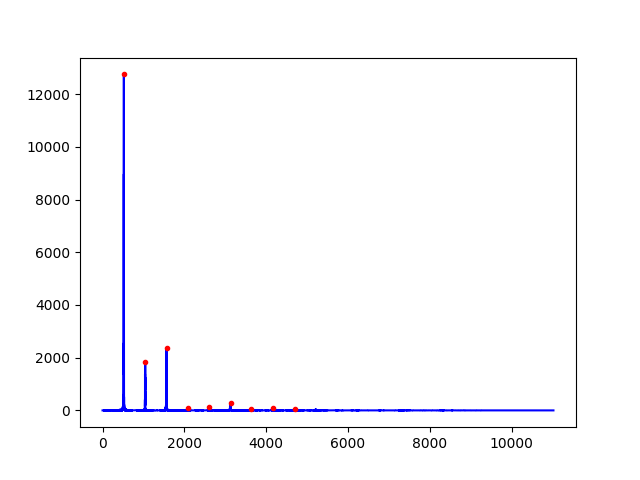
\includegraphics[scale=0.7]{flute-harmonics.png}
    \caption{Harmonics of the flute}
    \label{fig:my_label}
\end{figure}


\begin{table}[h!]
\begin{tabular}{|l|l|l|l|}
\hline
&n&	fn	&An\\
\hline

\checkmark &1&	246.11	&3561.42\\
\checkmark &2&	492.23	&7388.57\\
\checkmark &3&	737.96	&1010.52\\
\checkmark &4&	984.83	&1404.65\\
\checkmark &5&	1230.94	&559.03\\
\checkmark &6&	1477.80	&1447.17\\
\checkmark &7&	1723.92	&658.62\\
\checkmark &8&	1967.78	&685.11\\
\checkmark &9&	2216.52	&532.85\\
\hline
\end{tabular}
\caption{Violin}
\end{table}


\begin{figure}[!htbp]
    \centering
    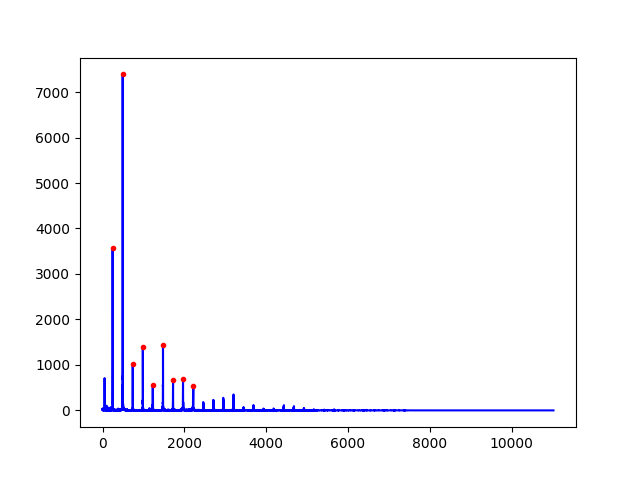
\includegraphics[scale=0.7]{violin-harmonics.png}
    \caption{Harmonics of the violin}
    \label{fig:my_label}
\end{figure}
\begin{table}[h!]
\begin{tabular}{|l|l|l|l|}
\hline
&n&	fn	&An\\
\hline

\checkmark &1&	184.41	&1499.67\\
\checkmark &2&	371.83	&1215.52\\
\checkmark &3&	557.24	&1269.36\\
&4&	741.65	&93.65\\
&5&	928.06	&105.03\\
&6&	1113.47&	65.64\\
&7&	1300.89&	127.71\\
&8&	1486.30&	65.40\\
&9&	1673.72&	123.68\\

\hline
\end{tabular}
\caption{Guitar}
\end{table}



\begin{figure}[!htbp]
    \centering
    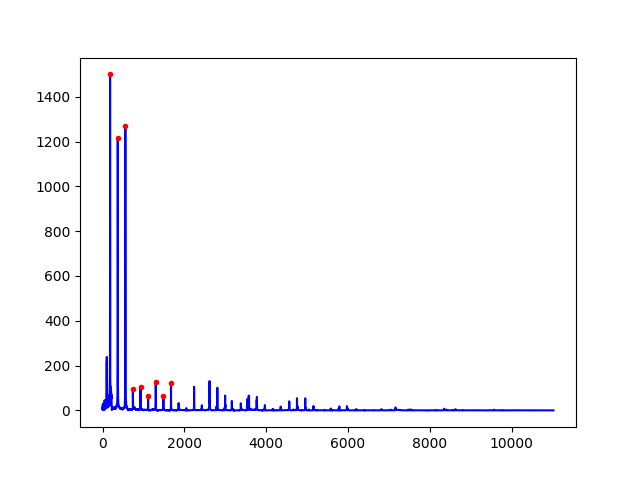
\includegraphics[scale=0.7]{guitar-harmonics.png}
    \caption{Harmonics of the guitar}
    \label{fig:my_label}
\end{figure}


\subsection{Insights}

\subsubsection{The sound file is not 100\% uniform throughout the time period. Can we crop the sound file for better accuracy?}

\begin{figure}[!htbp]
\minipage{0.32\textwidth}
  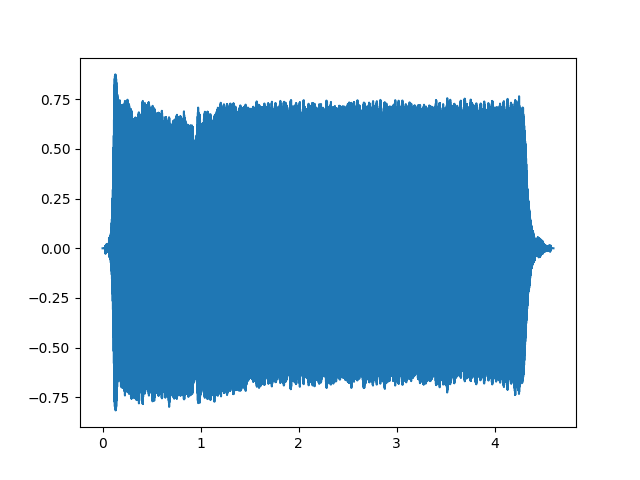
\includegraphics[width=\linewidth]{flute-timeSeries.png}
  \caption{Flute time series}\label{fig:a1}
\endminipage\hfill
\minipage{0.32\textwidth}
  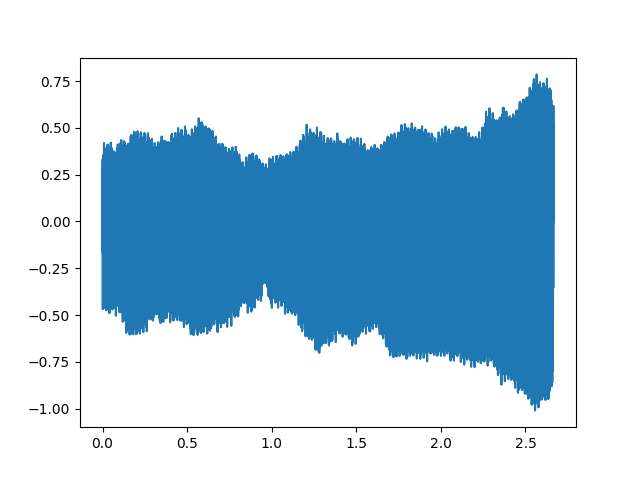
\includegraphics[width=\linewidth]{violin-timeSeries.png}
  \caption{Violin time series}\label{fig:a2}
\endminipage\hfill
\minipage{0.32\textwidth}%
  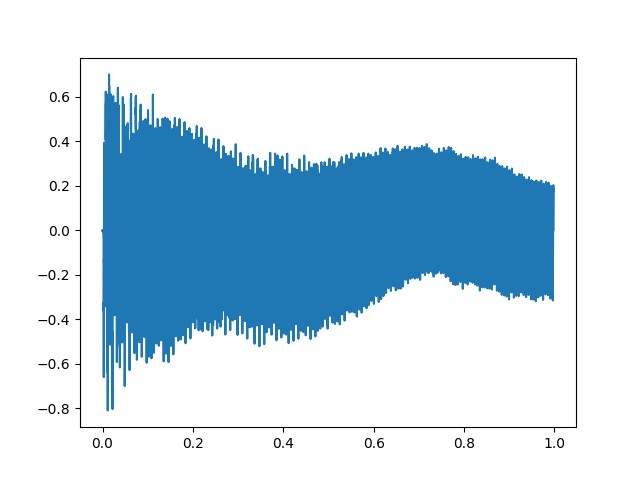
\includegraphics[width=\linewidth]{guitar-timeSeries.png}
  \caption{Guitar time series}\label{fig:a3}
\endminipage
\end{figure}

Time series images (\ref{fig:a1},\ref{fig:a2},\ref{fig:a3}) shows that violin and guitar are not giving the same pattern through out the file. But manually cropping this prevents the algorithm from being automatic. The refining part of the algorithm is used to handle this issue.

\begin{figure}[!htbp]
\minipage{0.32\textwidth}
  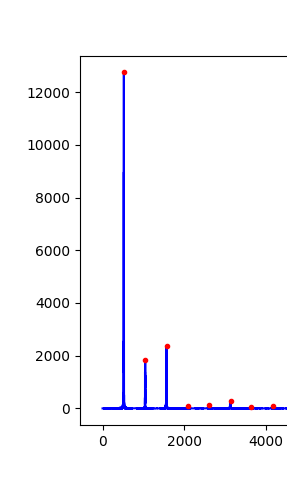
\includegraphics[width=\linewidth]{flute-harmonics-cropped.png}
  \caption{Flute harmonics}\label{fig:b1}
\endminipage\hfill
\minipage{0.32\textwidth}
  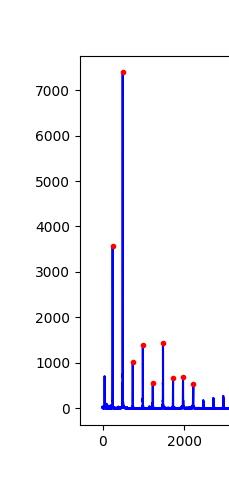
\includegraphics[width=\linewidth]{violin-harmonics-cropped.png}
  \caption{Violin harmonics}\label{fig:b2}
\endminipage\hfill
\minipage{0.32\textwidth}%
  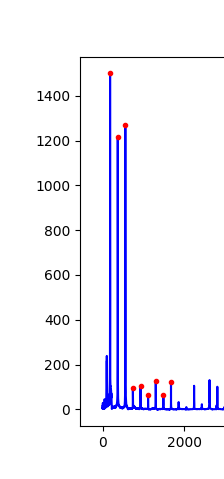
\includegraphics[width=\linewidth]{guitar-harmonics-cropped.png}
  \caption{Guitar harmonics}\label{fig:b3}
\endminipage
\end{figure}

This figures (\ref{fig:b1},\ref{fig:b2},\ref{fig:b3}) shows how the first peak of the Flute is considered as the fundamental frequency (marked by a red dot) while the first peak of other two instruments are discarded by the algorithm. This is done by \textbf{ALGORITHM 3} without being explicitly programmed to look for the noise only in this region. This solution is more generalized.


\subsubsection{The harmonics might have slight shifts from the expected frequencies. How are they handled?}


\begin{figure}[!htbp]
\minipage{0.32\textwidth}
  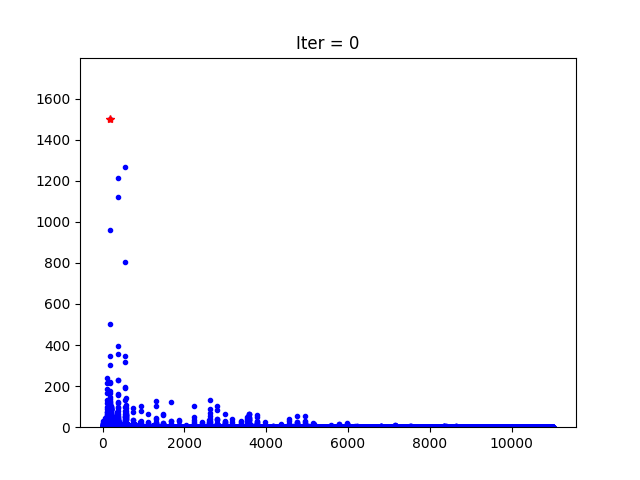
\includegraphics[width=\linewidth]{partial-finding-00.png}
  \caption{Algorithm 2 iteration 0}\label{fig:c1}
\endminipage\hfill
\minipage{0.32\textwidth}
  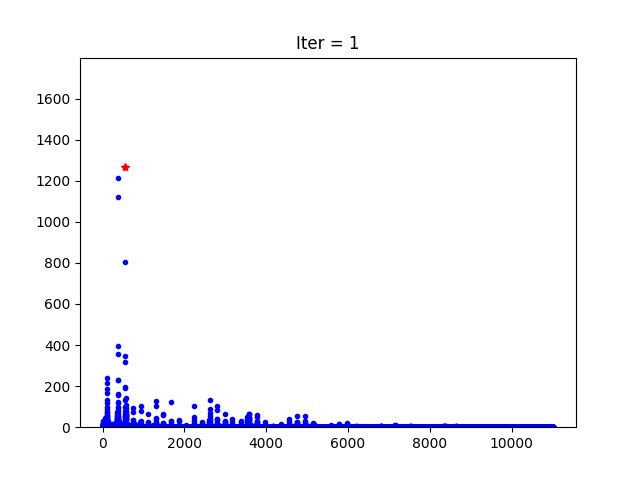
\includegraphics[width=\linewidth]{partial-finding-01.png}
  \caption{Algorithm 2 iteration 1}\label{fig:c2}
\endminipage\hfill
\minipage{0.32\textwidth}%
  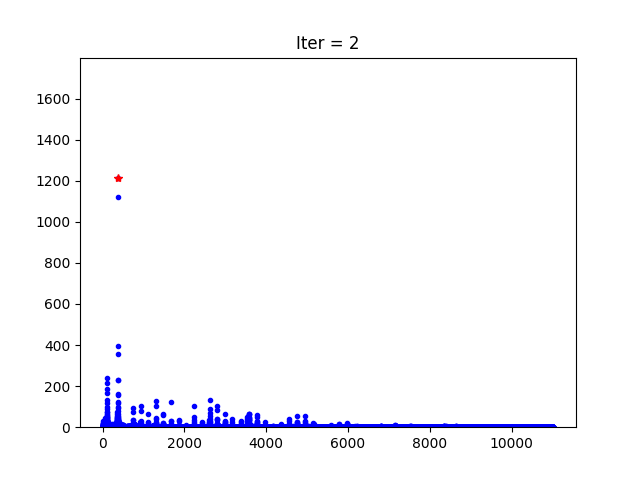
\includegraphics[width=\linewidth]{partial-finding-02.png}
  \caption{Algorithm 2 iteration 2}\label{fig:c3}
\endminipage
\end{figure}

The peaks in the frequency spectrum are not impulse like functions. They are spread out in a small window of frequency. This issue is handled in \textbf{ALGORITHM 2} by clearing out the neighbourhood of the peak before finding the next one. This is shown in figures \ref{fig:c3}, \ref{fig:c2} and \ref{fig:c3}



\section{Written question}
\subsection{What is the importance of Fourier transform with relation to digital music (200 words)}
Fourier transform is a mathematical tool capable of transforming a signal in the time series (music in the context of this project) to its counterpart in the frequency domain. The transform itself will generaly project any such signal and might give a dense frequency spectum throughout the frequency domain. These spectrums are difficult to analyze with infinite accuracy due tot he obvious limitations of computing (while approximations are possible). But when the time series signal is periodic (which is characterized by a fundamental period $T_0$) the corresponding frequency spectrum becomes very sparse (having zeros throuhout the spectrum except for a few specific frequencies known as harmonics).\cite{dict-music}


Music is generally periodic signals (at least periodic for a small time period). The fourier transform of of music signals is informative (we can easily deduce what note is being played), interpretable (since most components are zero, easy to understand) and manipulatable (eg: we can do filtering easily). When it comes to digital music (which is music sampled at discrete points in time at discrete representable floating point numbers) the fourier transform could be used for common purposes like compression, noise removal, enhancement, synthesis and transmission. Some uncommon usecases of the transform could be source separation, instrument identification, genre identification and vocal quality evalation.


\subsection{What is timbre?}
The basic way of characterizing the music (sound) is by it's frequency (fundamental -- smallest among harmonics or dominant -- highest amplitude) and amplitude. But these measures can be the same for any instrument playing the same note at same frequency. Obviously, human ear can find a difference. Timbre is an attempt to characterize this difference. \cite{timbre-pitch},\cite{harvard}

Timbre is also known as the tone quality. This is mathematically characterized by the frequency components of the sound in all the harmonics. For example, two instruments can have the same dominant frequency but very different amplitudes at other overtones. In a way, if it was not for timbre, all musical instruments will be equivalent to tuning forks.

\subsection{What is the fundamental frequency of a waveform?}
Fundamental frequency is the smallest frequency among the harmonics (other harmonics being overtones, who are integer multiples of the fundamental frequency). Fundamental frequency is also the time period of the periodic signal (in digital music, the signal is considered to be periodic at least over a small period of time.)



\subsection{What do you understand by harmonic partials and in-harmonic partials?}
Consider that there is a time series $f_{(t)}$ which can be written as a summation of sinusoidals as
$$f_{(t)} = \sum_{n=0}^{n=N}{A_nsin(2\pi f_nt)} ; \textrm{ where } A_n \neq 0 $$. These $f_n$ s can take any value. 

Assume that the function is periodic with a time period $T_0$ such that $$f_{(t)}=f_{(t+kT_0)} ; \textrm{ for } k \in \mathbb{Z} $$ 

The fundamental frequency $f_0$ would be $f_0 = \frac{2\pi}{T_0}$. The positive integer multiples of $f_0$ can be written as $\{kf_0 ; k \in \mathbb{Z}^+ \}$
\\ \\
\begin{center}
    
\begin{tabular}{c|c}
\hline
     Harmonic partials& $A_n sin(2\pi f_n t)$ for  $f_n \in \{kf_0 ; k \in \mathbb{Z}^+ \}$\\
    In harmonic partials& $A_n sin(2\pi f_n t)$ for  $f_n \notin \{kf_0 ; k \in \mathbb{Z}^+ \}$\\
\end{tabular}
\end{center}


\subsection{What is the relationship of harmonics partials and timbre?}
If there is only one harmonic partial -- dominant frequency $(N=1)$ the instrument will be playing the pure note. But the existence of a large number of harmonic partials $(N >> 1)$ gives rise to timbre.






\bibliographystyle{unsrt}
\bibliography{references}


\end{document}